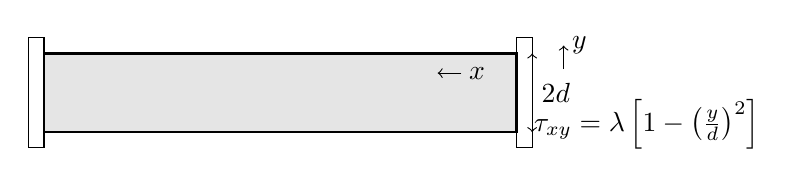
\begin{tikzpicture}
    % Draw the beam
    \fill[gray!20] (0,0) rectangle (6,1);
    \draw[thick] (0,0) rectangle (6,1);
    
    % Add end supports
    \draw (-0.2,-0.2) rectangle (0,1.2);
    \draw (6,-0.2) rectangle (6.2,1.2);
    
    % Dimension line for height
    \draw[<->] (6.2,0) -- (6.2,1);
    \node at (6.5,0.5) {$2d$};
    
    % Label for x-axis
    \node at (5.5,0.75) {$x$};
    \draw[->] (5.3,0.75) -- (5,0.75);
    
    % Label for y-axis
    \node at (6.8,1.1) {$y$};
    \draw[->] (6.6,0.8) -- (6.6,1.1);
    
% Add equation text
    \node[anchor=west] at (6.1,0.1) {$\tau_{xy} = \lambda \left[ 1 - \left( \frac{y}{d} \right)^2 \right]$};
\end{tikzpicture}
